\documentclass[12pt,a4paper]{article}
\usepackage[utf8]{inputenc}
\usepackage[german]{babel}
\usepackage[T1]{fontenc}
\usepackage{amsmath}
\usepackage{amsfonts}
\usepackage{amssymb}
\usepackage{graphicx}
\usepackage[left=2.5cm,right=2.5cm,top=2cm,bottom=2cm]{geometry}
\usepackage{float}
\author{Gruppe C14 \\ Julián Häck, Martin Koytek, Lars Wenning, Erik Zimmermann}
\begin{document}
\section{Vermessung der Schallgeschwindigkeit durch Variation der Frequenz}
\subsection{Versuchsberschreibung}
In diesem Versuch werden wir die Schallgeschwindigkeit aus der Steigung der Geraden 
\begin{equation}
f_n = \frac{n\cdot v}{2\cdot L}
\end{equation}
bestimmen. Dabei steht $f_n$ für die Resonanzfrequenzen, n für die Vielfache, v für die Schallgeschwindigkeit und L für die Länge des Rohres. Dafür vermessen wir zunächst grob die Resonanzfrequenzen.
Danach werden wir das gleiche noch einmal genau wiederholen, aber mit deutlich mehr Messpunkten um die jeweiligen Resonanzfrequenzen (siehe Bild), insgesamt 3 mal.

\subsection{Versuchsaufbau und Durchführung}
Verwendete Geräte:
\begin{itemize}
\item Frequenzgenerator
\item Sensor-Cassy
\item Richtmikrofon
\item Lautsprecher
\item Rohr ($0.425\, m \pm 0.001\,$ m (Messfehler auf Massband))
\item Massband ($\sigma_{Massband} = 0.001\, m$)
\end{itemize}
Wir haben unser Cassy mit folgenden Einstellungen verwendet:
\begin{itemize}
\item Kanal A / Spannung UA1 / $-10..10\, V$ /
\item Kanal B / Timerbox / Frequenz fb1(E) / $5000\, Hz$ / Torzeit: $1\, s$
\item manuelle Messung
\item Darstellung: X-Achse fb1 / Y-Achse Ua1
\end{itemize}
Den Frequenzgenerator haben wir wie folgt eingestellt:
\begin{itemize}
\item Signalform / $\sim$ (Sinusschwingung)
\item Bereich / $x1k (0.2 - 2.4 x 1\, $kHz$)$
\item $\sigma_f = 10\,$Hz (Abschätzung durch ungenaue Feinabstimmung, gerätbedingt)
\item Offset / 0
\item Amplitude / mittig
\end{itemize}
\begin{figure}[H]
\centering
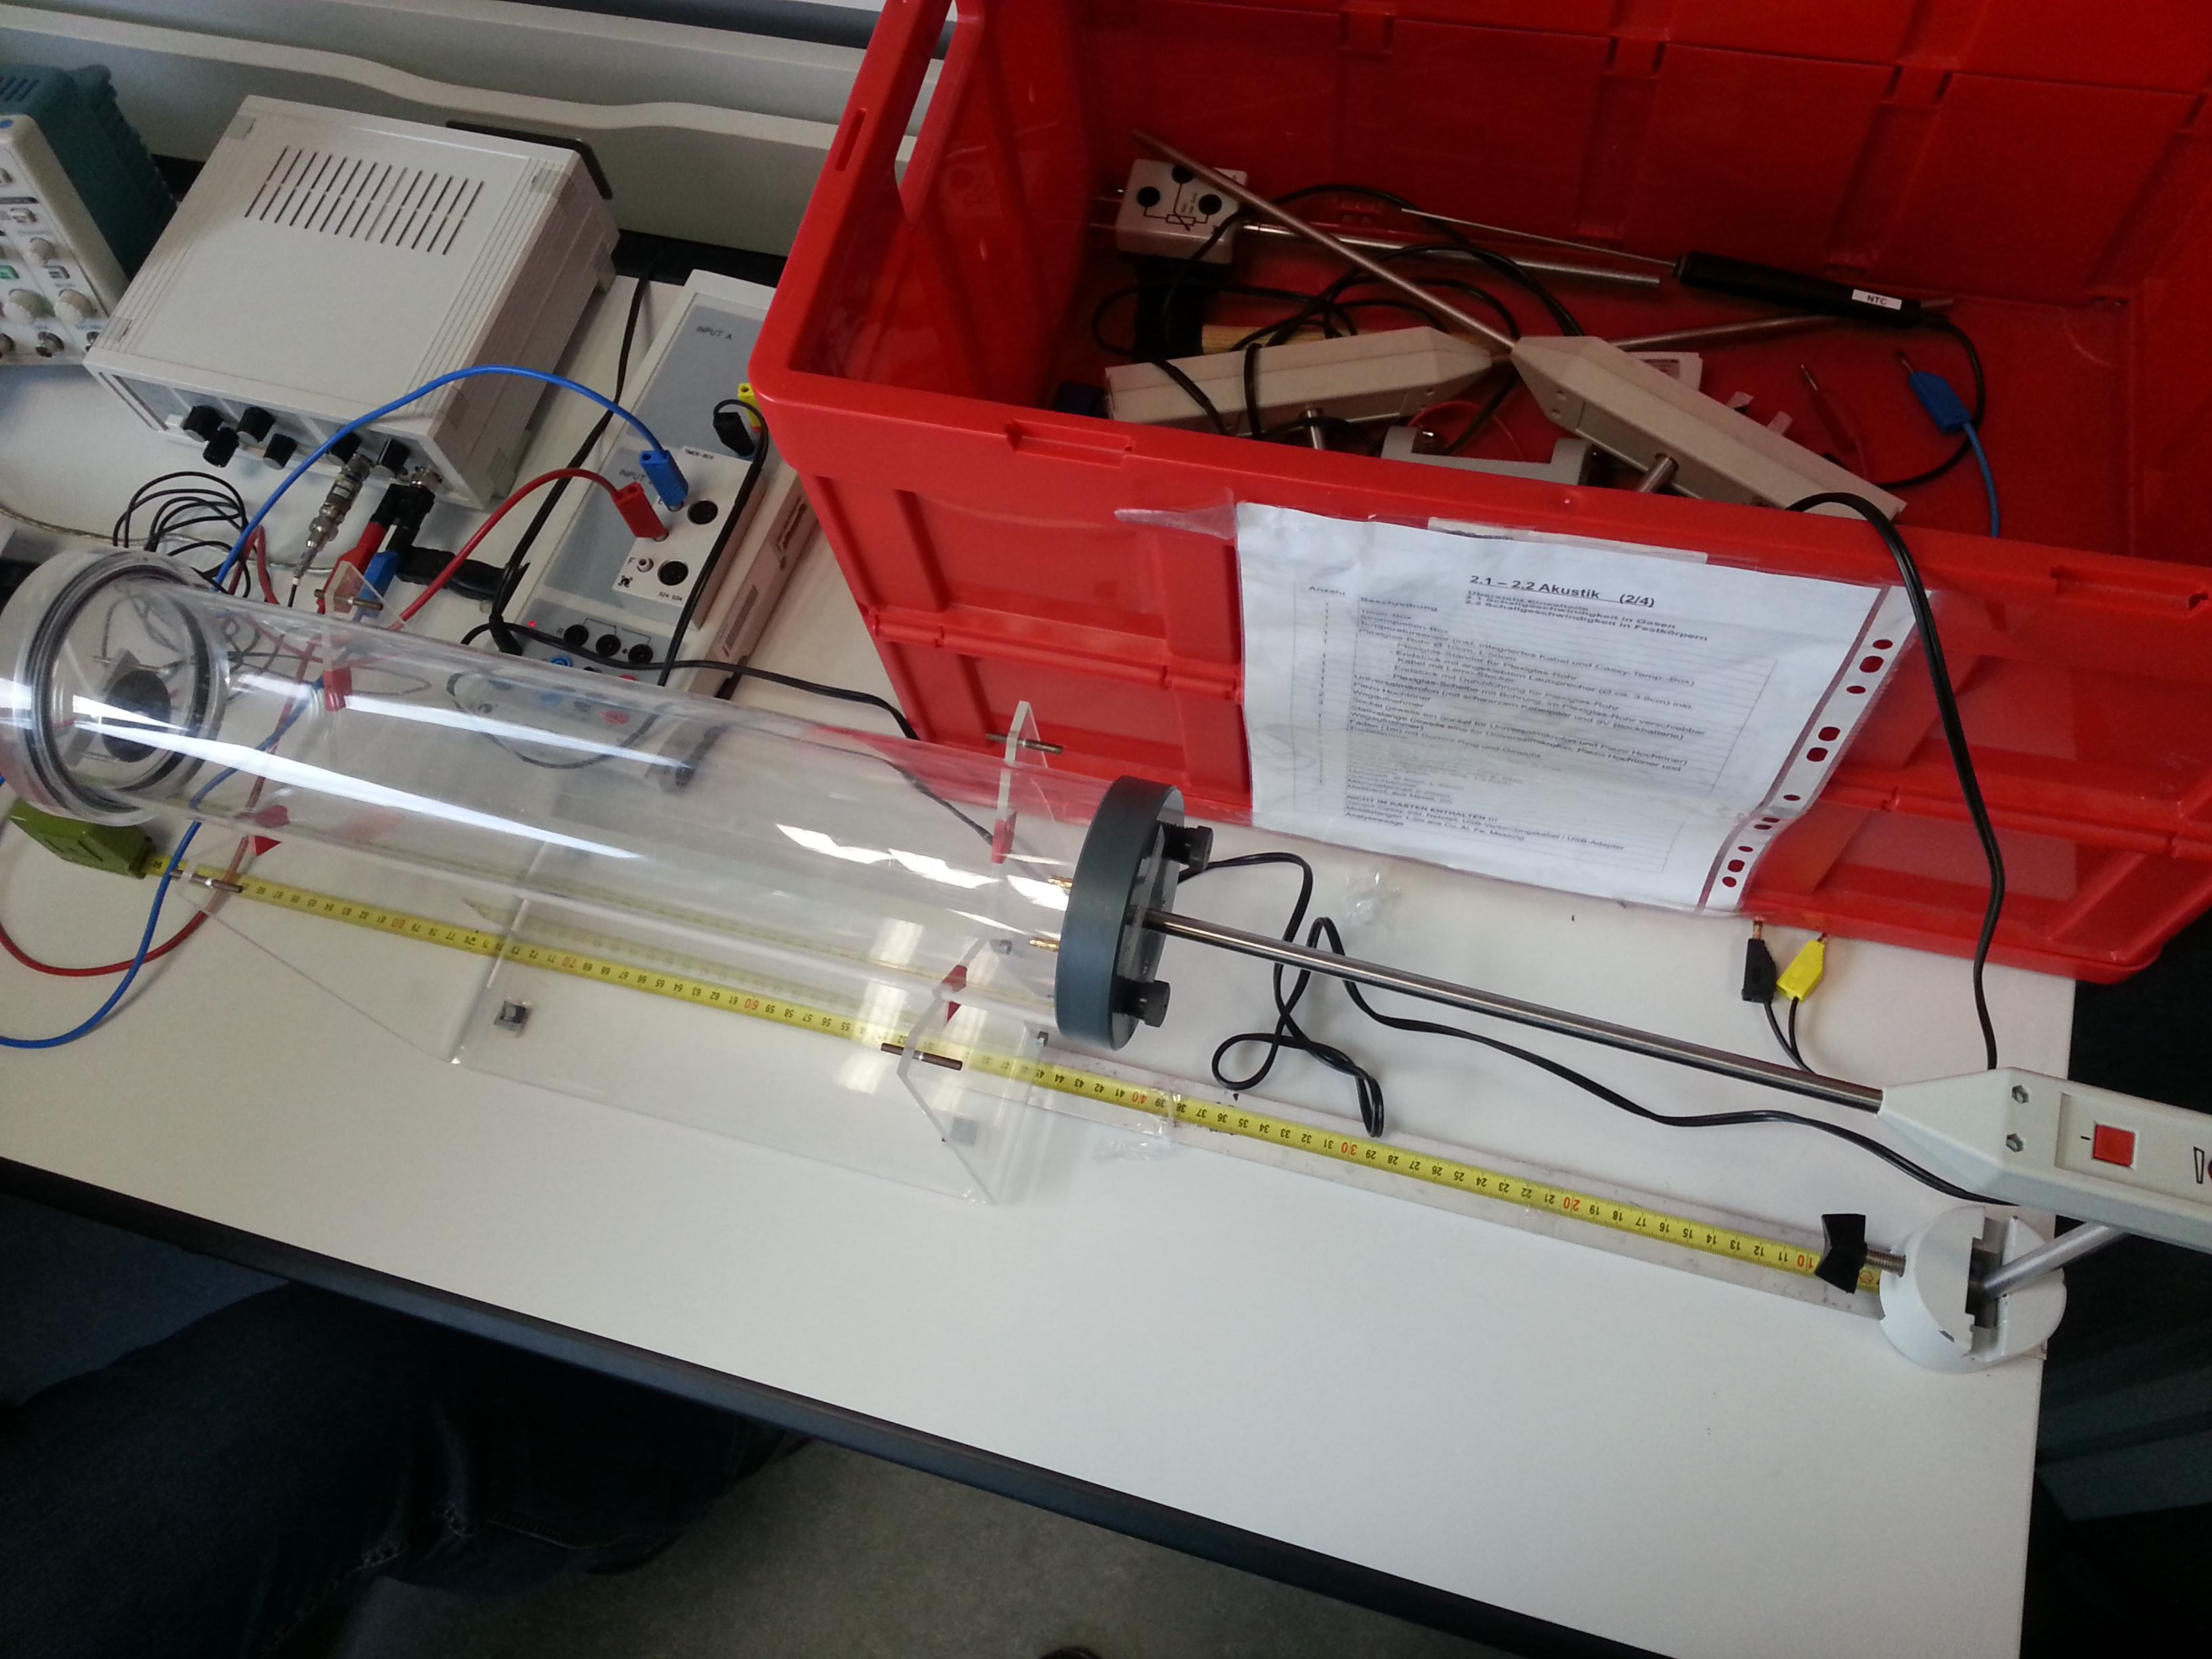
\includegraphics[scale=0.15]{Bilder/Frequenzvariation3.jpg}
\caption{Versuchsaufbau zur Messung der Schallgeschwindigkeit durch Variation der Resonanzfrequenzen}
\end{figure}
Zunächst haben wir grob die Resonanzfrequenz bestimmt:
\begin{figure}[H]
\centering
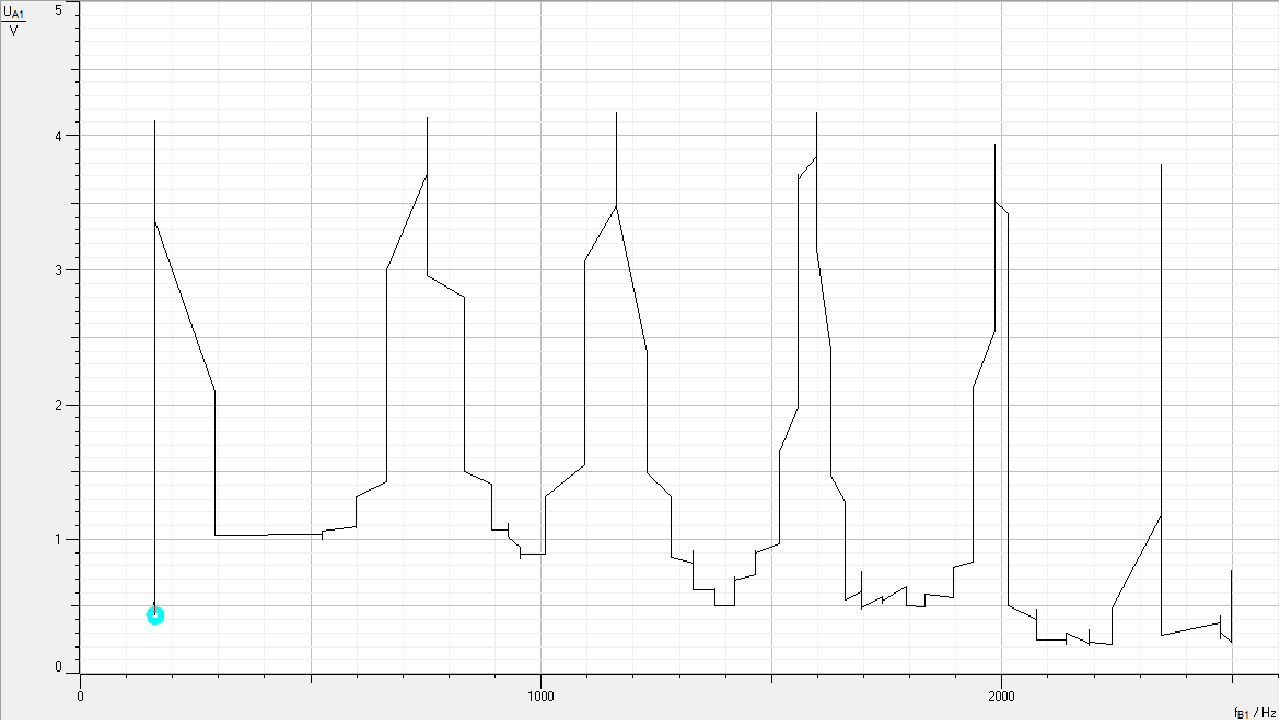
\includegraphics[scale=0.5]{Bilder/grobevermessung.png}
\caption{Grobe Vermessung der Resonanzfrequenzen - die deutlich ausgeprägten Peaks werden später genauer untersucht.}
\end{figure}
Danach haben wir an den oben zu sehenden Peaks das ganze noch mal mit mehr Messpunkten in drei Messungen gemessen:
\begin{figure}[H]
\centering
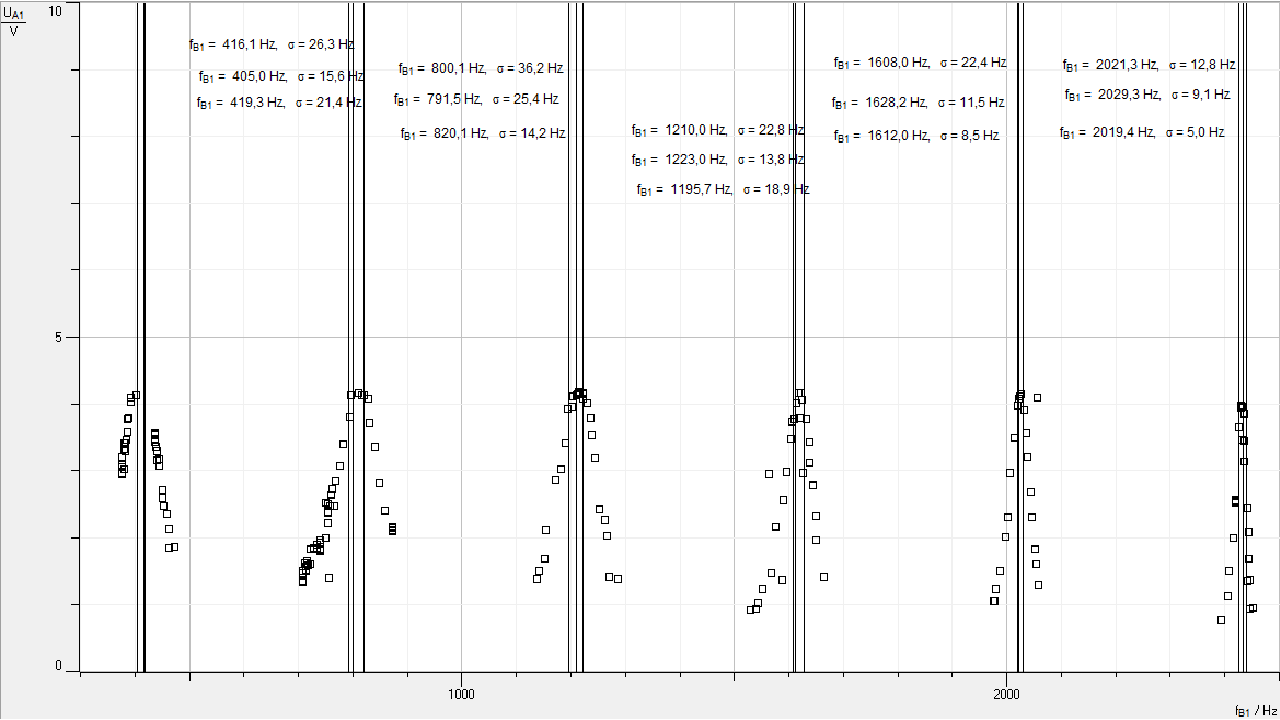
\includegraphics[scale=0.5]{Bilder/vermessung_variation_genau.png}
\caption{genaue Vermessung der Peaks an einer Beispiel Messung}
\end{figure}
Die sich daraus ergebenen Daten sind unter Rohdaten aufgeführt.
\subsection{Versuchsauswertung}
\subsubsection{Rohdaten}
\begin{table}[H]
\begin{tabular}{c|c|c|c|c|c|c}
vermutete Resonanzfrequenz & 400 & 800 & 1200 & 1600 & 2000 & 2400 \\ 
\hline 
Peak Messung I & 416.0 & 822.5 & 1210.0 & 1608.0 & 2031.1 & 2433.4 \\  
$asym_r$ Peak Messung I & 417.0 & 826.8 & 1212.6 & 1629.6 & 2041.4 & 2443.7 \\  
$asym_l$ Peak Messung I & 404.9 & 798.2 & 1190.0 & 1573.9 & 2019.3 & 2425.5 \\ 
\hline 
Peak Messung II & 420.7 & 822.1 & 1210.9 & 1620.0 & 2037.2 & 2446.7 \\  
$asym_r$ Peak Messung II & 423.0 & 836.4 & 1216.5 & 1631.3 & 2047.8 & 2467.3 \\ 
$asym_l$ Peak Messung II & 404.3 & 797.5 & 1194.0 & 1612.3 & 2013.8 & 2421.3 \\ 
\hline 
Peak Messung III & 416.1 & 800.1 & 1210.0 & 1612.0 & 2019.4 & 2433.4 \\  
$asym_r$ Peak Messung III & 419.3 & 820.1 & 1223.0 & 1628.2 & 2029.3 & 2439.2 \\  
$asym_l$ Peak Messung III & 405.0 & 791.5 & 1195.7 & 1608.0 & 2019.4 & 2425.5
\end{tabular}
\caption{Vermessung der Resonanzfrequenzen, wobei $asym_r$ und $asym_l$ die asymmetrische Peakvermessung in Cassy (alle Angaben in Hz)} 
\end{table}
Die Raumtemperatur betrug $23^{\circ}\, C$.
\subsubsection{Transformation der Rohdaten}
\begin{table}[H]
\begin{tabular}{c|c|c|c|c|c|c}
vermutete Resonanzfrequenz & 400 & 800 & 1200 & 1600 & 2000 & 2400 \\ 
\hline 
$\bar{M}$ & 412.92 & 812.80 & 1206.97 & 1614.70 & 2030.07 & 2437.33 \\ 
\hline 
$\sigma_{\bar{M}}$ & 6.94 & 16.00 & 11.16 & 18.21 & 10.90 & 14.32 \\ 
\end{tabular}
\caption{Mittelwerte und deren Fehler (alle Angaben in Hz)} 
\end{table}
Nachdem wir die Mittelwerte auf die einzelnen Resonanzfrequenzen und den Fehler auf den Mittelwert  berechnet haben werden wir diese Daten für eine Lineare Regression verwenden. Wir fitten eine Funktion der Form $Fit = m\cdot x + b$.
\begin{equation}
\bar{M} = \frac{\sum_{i=1}{n}{X_i}}{n}
\end{equation}
und
\begin{equation}
\sigma_{\bar{M}} = \frac{\sqrt{\frac{\sum_{i=1}^{N}({X_i-\bar{M}})^2}{N-1}}}{\sqrt{N}}
\end{equation} 
Dabei tragen wir unsere Resonanzen gegen die Mittelwerte auf.
\begin{figure}[H]
\centering
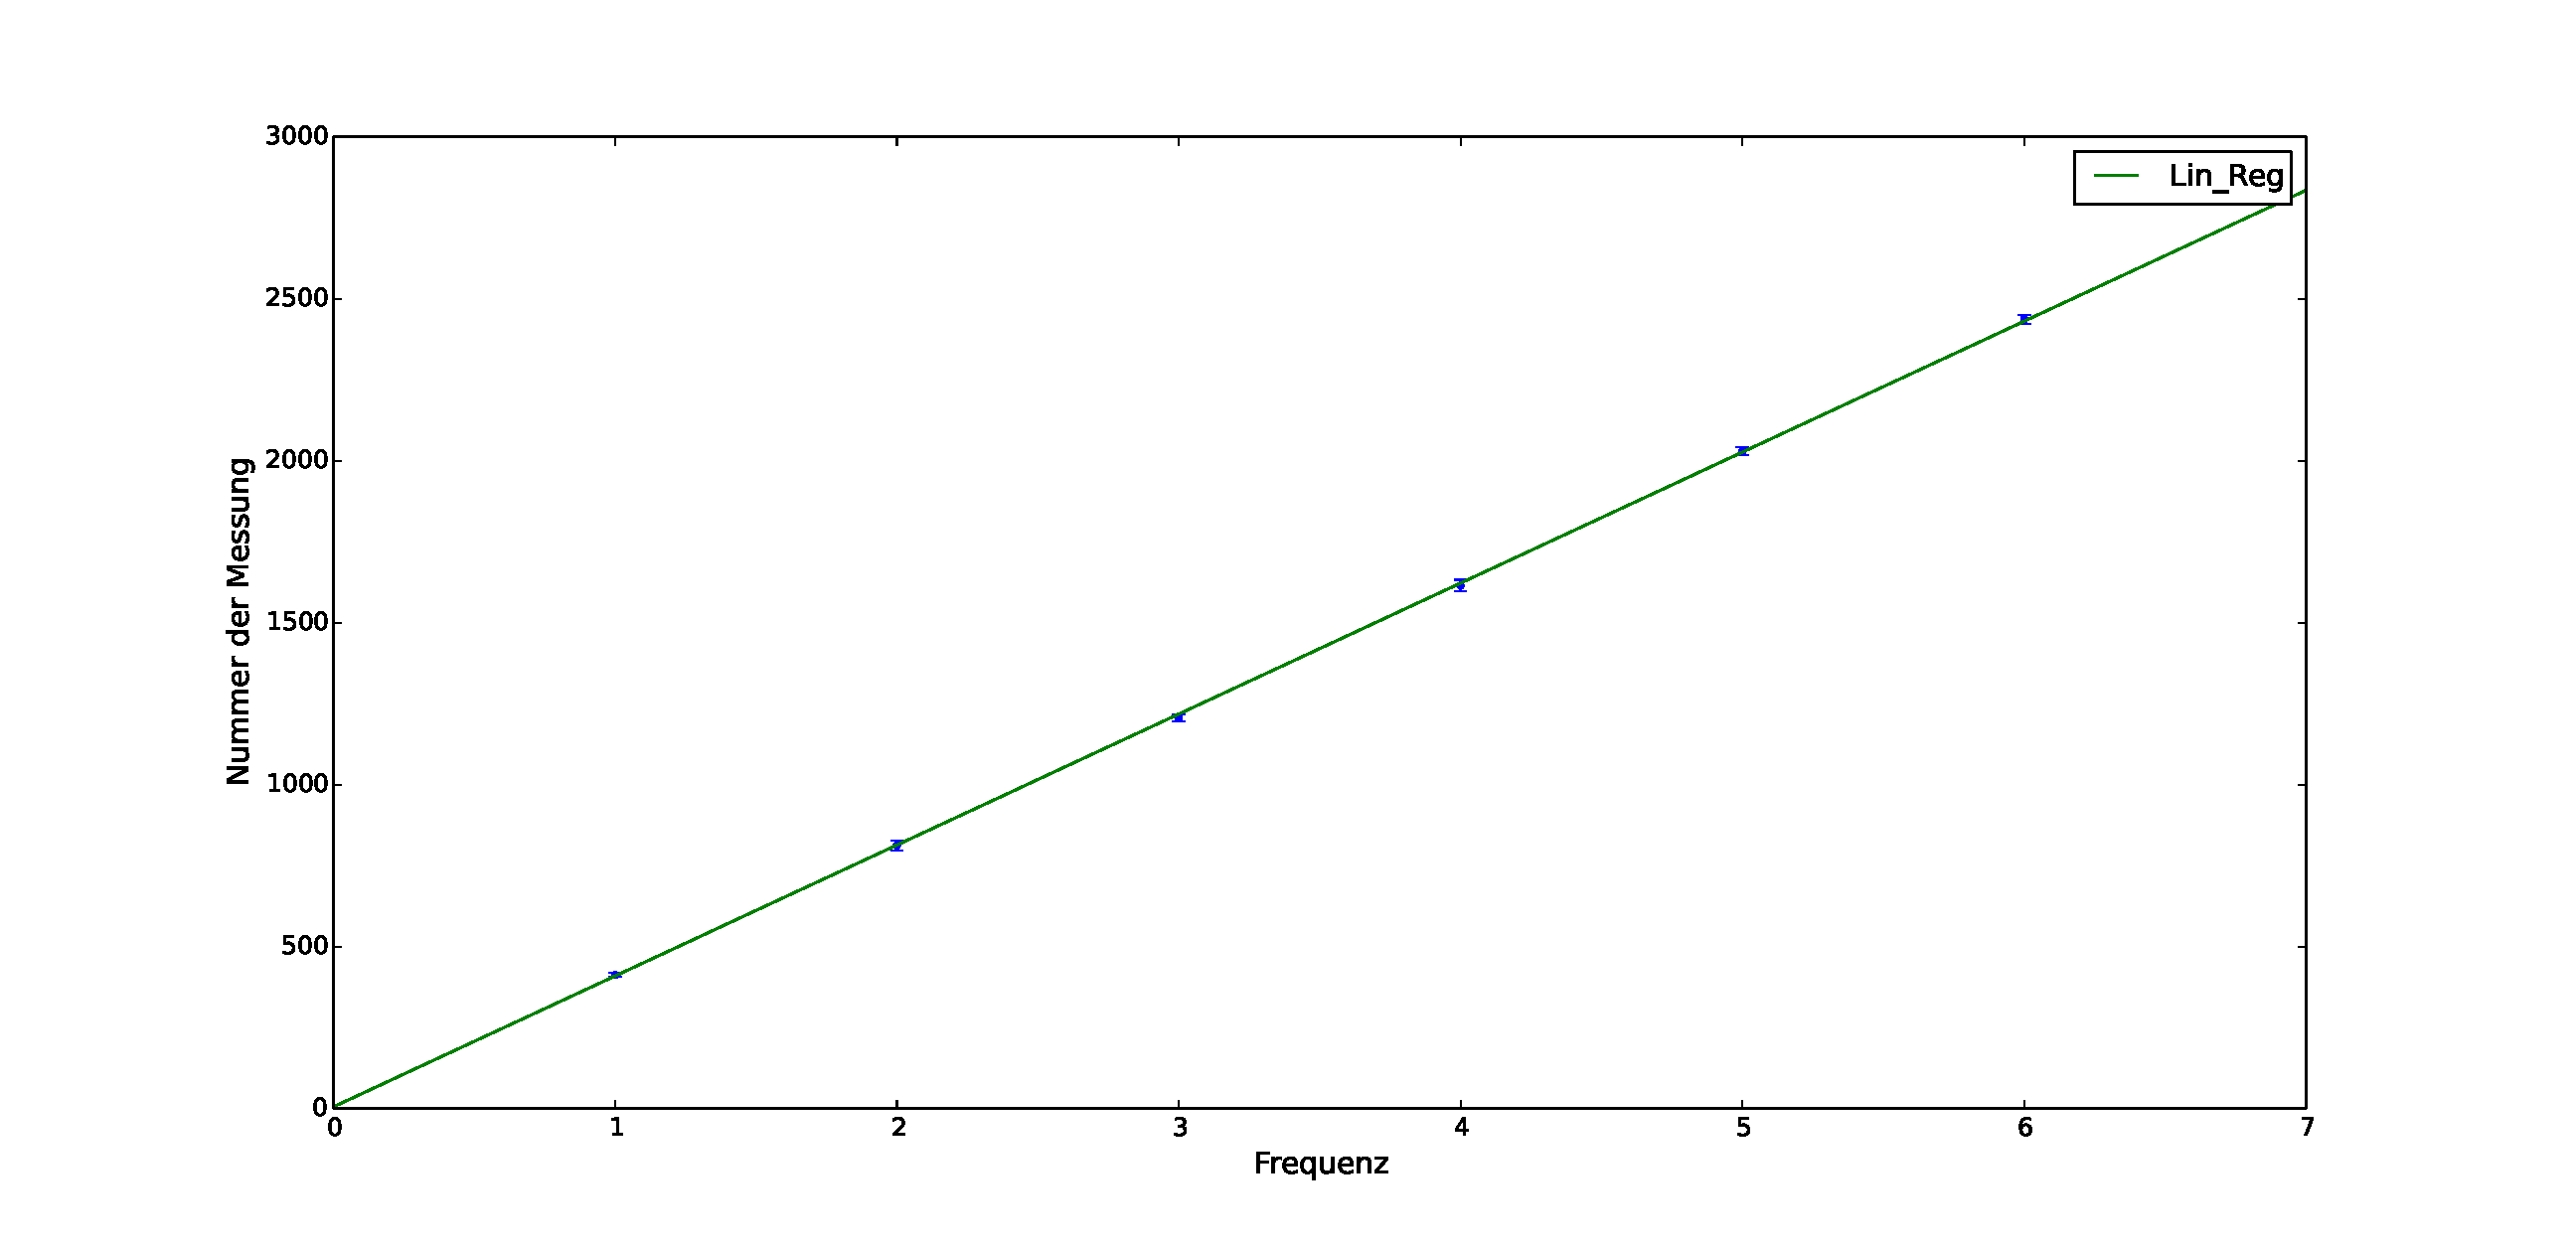
\includegraphics[scale=0.3]{Bilder/linreg_variation.eps}
\caption{Lineare Regression, die Steigung gibt $\frac{v_{Schall}}{2\cdot L}$ zurück}
\end{figure}
Mit einem $\chi^2 = 0.43$ ist unsere Anpassung in einem akzeptablen Rahmen. Das spiegelt sich auch in unserem Residuenplot wieder:
\begin{figure}[H]
\centering
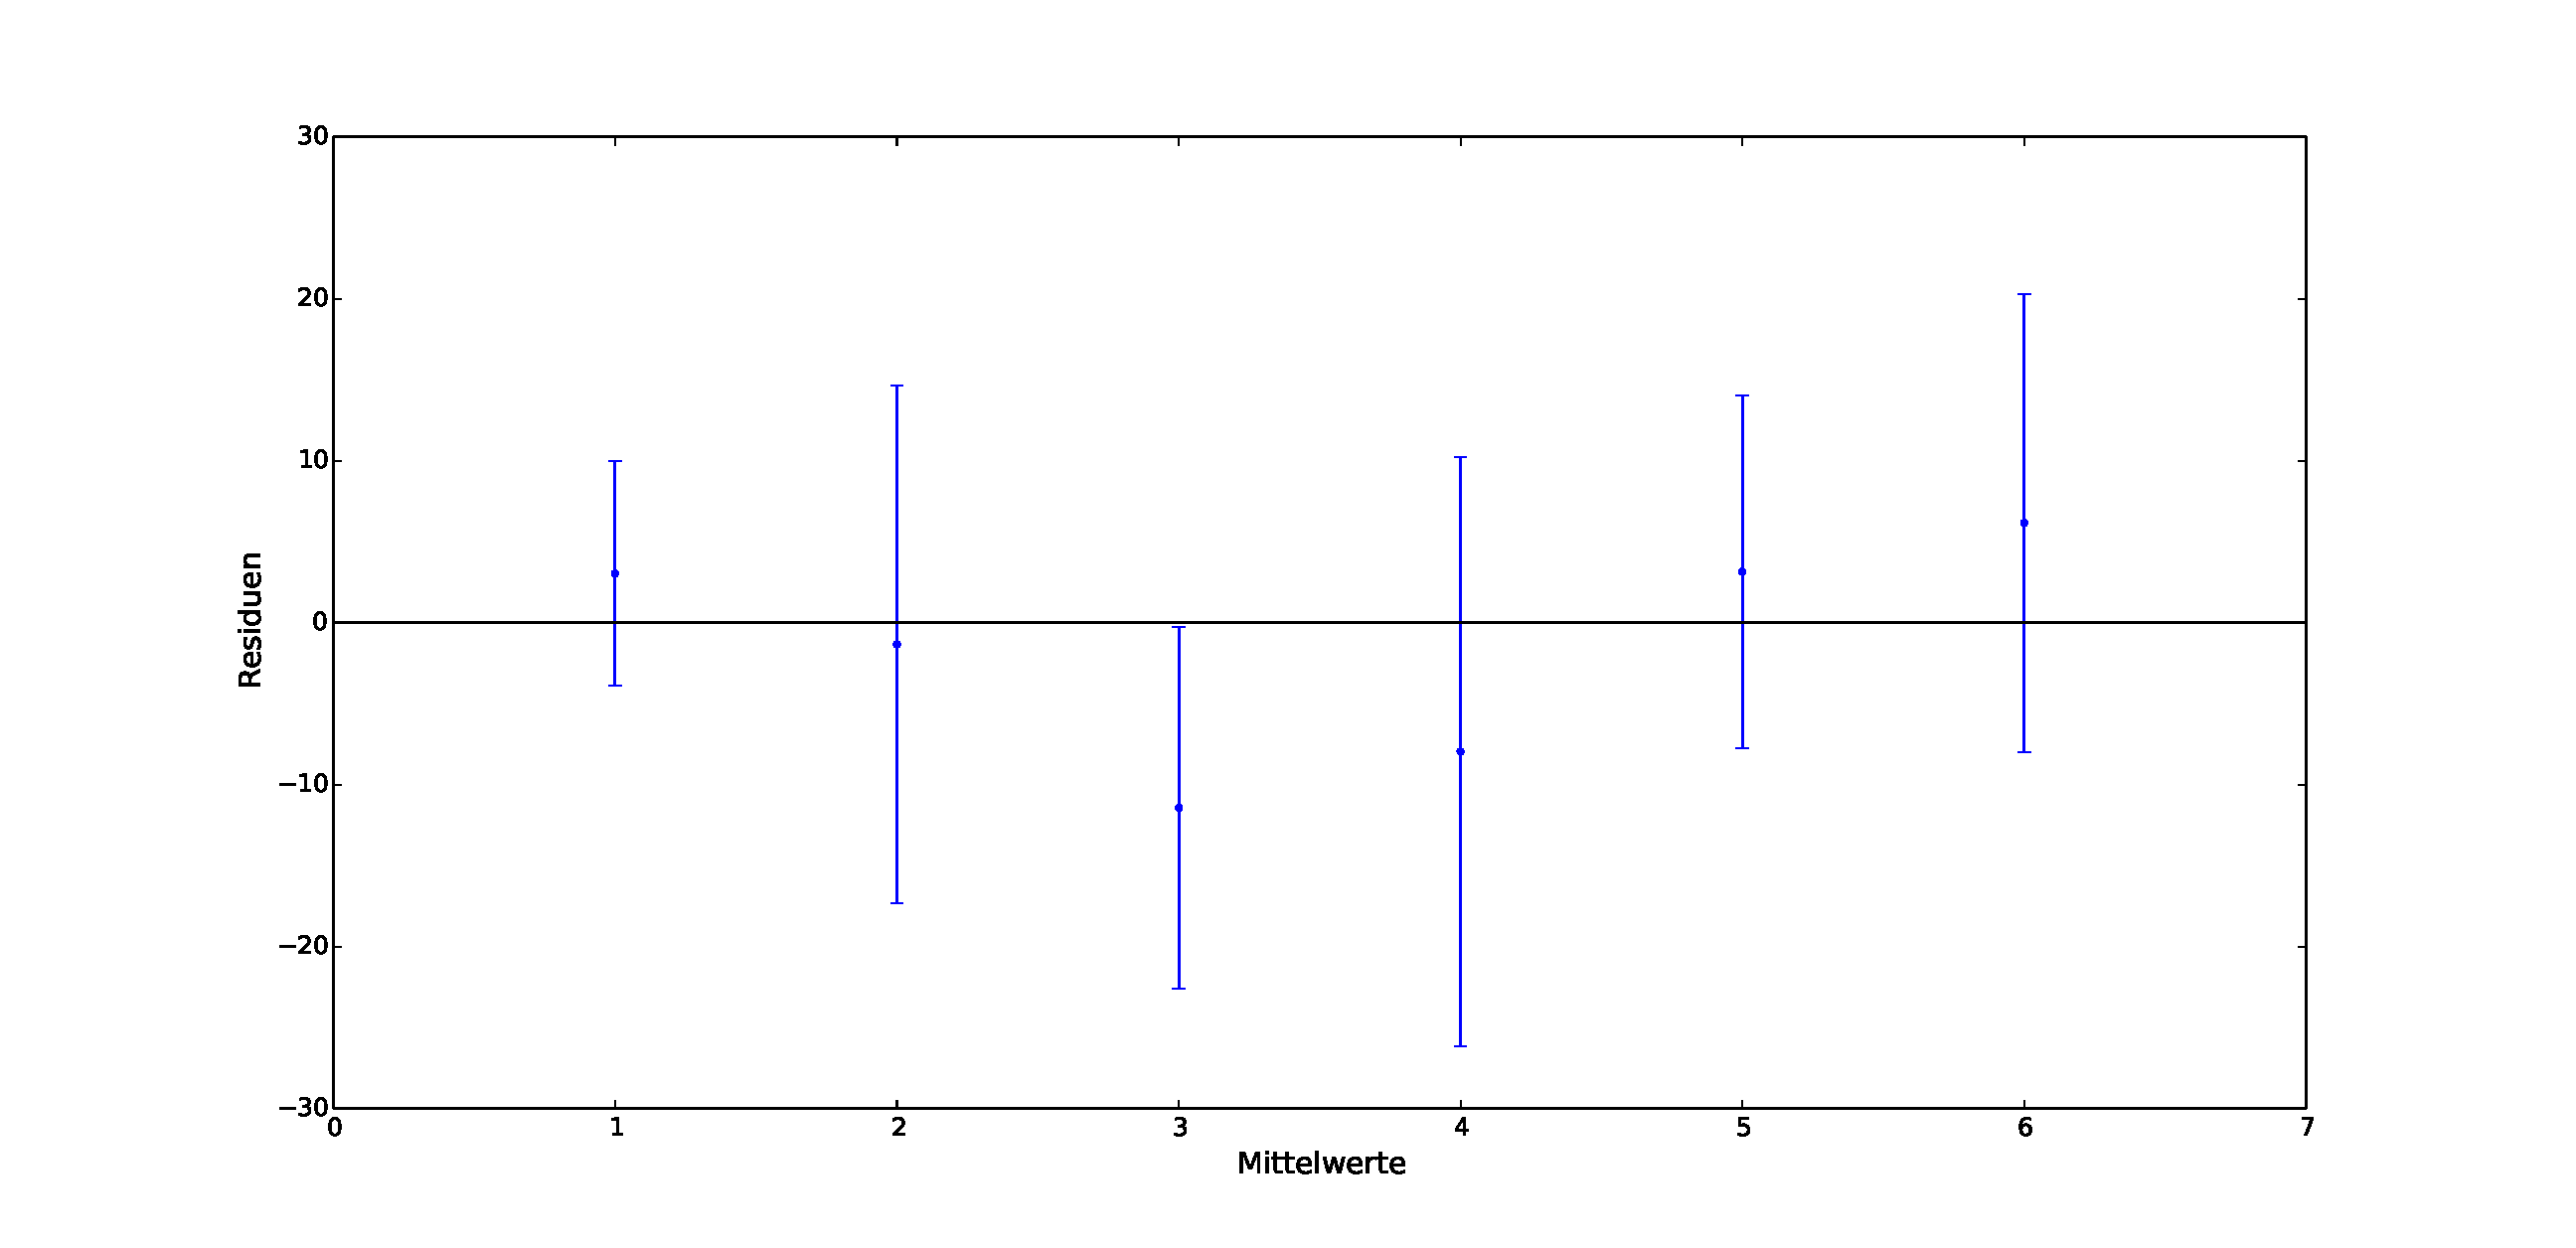
\includegraphics[scale=0.3]{Bilder/Residuen_Variation_Frequenzen.eps}
\caption{Residuenplot (Werte-Fit), zeigt Güte der Anpassung}
\end{figure}
Die Residuen streuen gleichverteilt um 0. 5 von 6 Werten schneiden die Nulllinie mit ihren Fehlerbalken, das entspricht $83.3\%$ der Werte die innerhalb von einem $\sigma$ den Sollwert schneiden. 
Die Steigung der Linearen Regression gibt uns die Schallgeschwindigkeit mit dem Faktor $\frac{1}{2\cdot L}$ wieder, wie auch schon in
\begin{equation}
f_n = \frac{n\cdot v}{2\cdot L}
\end{equation}
zu sehen ist.
Die Fehler auf die Längenmessung und die Fehler auf die Mittelwerte unserer Resonanzfrequenzen haben wir wie folgt fortgepflanzt:
\begin{equation}
\sigma_v = \sqrt{f_R^2\cdot\sigma_{\lambda}^2 + \lambda^2\cdot\sigma_f^2}
\end{equation}
mit
\begin{equation}
\sigma_{\lambda} = \sigma_{\bar{M}}\cdot\sqrt{2}
\end{equation}
$\bar{M}$ und $\sigma_{\bar{M}}$ haben wir erhalten durch:
\begin{equation}
\bar{M} = \frac{\sum_{i=1}^{N}{X_i}}{N}
\end{equation}
und
\begin{equation}
\sigma_{\bar{M}}=\frac{\sqrt{\frac{\sum_{i=1}^{N}({X_i-\bar{M}})^2}{N-1}}}{\sqrt{N}}
\end{equation}
Nach der Korrektur erhalten wir einen Wert für $v$ von
\begin{equation}
v = 343.46 \pm 2.08\,\frac{m}{s}
\end{equation}.

\subsection{Fazit}
Unser Wert für $v_{Schall}$ liegt innerhalb eines $\sigma$ Abstand zum Literaturwert (bei $T = 20^{\circ}\,$C) $v_{lit}=343\,\frac{m}{s}$. Unsere Fehlerabschätzungen führen zu einem relativen Fehler auf $v$ von $0.58\%$, was, zusammen mit unserem $\chi^2 = 0.43$ und Residuenplot, der keine Systematiken aufweist, sondern eine gleichverteilte Streuung um 0 zeigt, auf eine sehr präzise Messung schließen lässt, mit der wir als Gruppe zufrieden sind.

\end{document}